\documentclass[a4paper,11.5pt,table]{article}
\usepackage[textwidth=170mm, textheight=230mm, inner=20mm, top=20mm, bottom=30mm]{geometry}
\usepackage[normalem]{ulem}
\usepackage[utf8]{inputenc}
\usepackage[T1]{fontenc}
\PassOptionsToPackage{defaults=hu-min}{magyar.ldf}
\usepackage[magyar]{babel}
\usepackage{amsmath, amsthm,amssymb, paralist, tikz, multirow, float}
\usetikzlibrary{arrows, positioning}

\usepackage{listings}
\lstset{
	language=C++, 
	basicstyle=\ttfamily, 
	keywordstyle=\color{blue}\ttfamily, 
	stringstyle=\color{red}\ttfamily,
	tabsize = 4
}

\usepackage{hyperref}

\begin{document}
	%%%%%%%%%%%RÖVIDÍTÉSEK%%%%%%%%%%
	\setlength\parindent{0pt}
	\def\<{<\hspace{0mm}<}
	
	\theoremstyle{definition}
	\newtheorem{note}{Megjegyzés}[subsection]
	%%%%%%%%%%%%%%%%%%%%%%%%%%%%%%%%%%%%%%%%%%%%%%%%%%%%%%%%%%%%%%%%%%%%%
	
	\begin{center}
		{\LARGE\textbf{C++}}
		
		{\Large Gyakorlat jegyzet}
		
		4. óra.
	\end{center}
	A jegyzetet \textsc{Umann} Kristóf készítette \textsc{Horváth} Gábor  előadásán. (\today)
	
	%TODO jobb és balérték
	\subsection{Tömbök átadása függvényparaméterként}
	Próbáljunk meg egy tömböt érték szerint átadni egy függvénynek!
	\begin{lstlisting}
#include <iostream>

void f(int t[])
{
	std::cout << sizeof(t) << std::endl;
}

int main()
{
	int t[] = {1,2,3,4,5};
	std::cout << sizeof(t) << std::endl;
	f(t);
}
	\end{lstlisting}
	Kimenet: \texttt{20 8} (ezen az implementáción)
	
	Bár mindkétszer azt hittünk hogy \texttt{t} tömb által foglalt méretét írattuk ki, és azt várnánk hogy a két szám ugyanaz lesz, a valóságban amikor azt érték szerint megpróbáljuk átadni, a \texttt{t} tömb átkonvertálódik a tömb elejére mutató pointerré.
	\begin{lstlisting}
void f(int t[8])
{
	std::cout << sizeof(t) << std::endl;
}
	\end{lstlisting}
	Ebben az esetben még mindig 8 lesz a második kiírt szám. Az a tanulság, hogy ha érték szerint akarunk átadni egy tömböt, ahelyett át fog konvertálódni pointerré. Az, hogy ezt szintaktikailag miért tehetjük meg mégis, hogy egy tömböt írunk oda mégis pointert kapunk, 
	\begin{center}
		\textit{,,az egy faszság.''}
		
		/Horváth Gábor/
	\end{center}
	\begin{note}
		Tömböt értékül adni a szabvány szerint nem is lehet: \texttt{int *t2[5] = t} nem helyes.
	\end{note}
	Korábban megismerkedtünk egy módszerrel, mely segítségével egy tömb méretét (elemszámát) paraméterátadás után is megőriztük:
	\begin{lstlisting}
#include <iostream>

void f(int *t, int size) //uj parameter!
{
	std::cout << sizeof(t) << std::endl;
}

int main()
{
	int t[] = {1,2,3,4,5};
	std::cout << sizeof(t) << std::endl;
	f(t, sizeof(t)/sizeof(t[0]));
}
	\end{lstlisting}
	\begin{note}
		Amennyiben c++11ben programozunk, érdemes az \texttt{std::array}-t használnunk, ami majdnem ugyanaz, mint egy tömb, legalább olyan hatékony, de nem tud pointerré változni és mindig tudja a méretét.
	\end{note}
	Ha szeretnénk egy tömböt egy darab paraméterrel átadni, megpróbálhatunk egy tömbre mutató pointert létrehozni. Azonban figyelni kell a szintaktikára, ha \texttt{int *t[5]}-t írunk, egy öt elemű intre mutató pointereket tároló tömböt kapunk.
	
	\medskip
	Ha valóban tömbre mutató mutatót szeretnék, így csinálhatjuk:
	\begin{lstlisting}
void g(int (*t)[5])
{
	std::cout << sizeof(t) << std::endl;
}
	\end{lstlisting}
	Azonban ez még mindig 8at fog kiírni (ezen az implementáción!), mert a \texttt{t} az egy sima mutató! Ahhoz, hogy megkapjuk, mire mutat, dereferálnunk kell, így a \texttt{sizeof} paraméterének \texttt{*t}-t kell megadni.
	\begin{note}
		Nyilván, ha refenreciával vennénk át \texttt{t}-t, az is hasonlóan nézne ki:\, \texttt{int (\&t)[5]}.
	\end{note}
	\medskip
	
	Ha megnöveljük a tömb méretét eggyel, akkor nem fordul le a kód, mert nem tud a g függvényben egy 5 elemű tömbre mutató mutató 6 elemű tömbre mutató mutatóvá konvertálódni.
	\begin{lstlisting}
int main()
{
	int a[6];
	g(a); //forditasi hiba!
	int b[5];
	g(b); //ok
}
	\end{lstlisting}
	
	\section{Literálok}
	\subsection{Karakterláncok}
	Mi lesz a \texttt{"Hello"} sztring típusa?
	\smallskip
	
	Egy konstans karakterekből álló 6 méretű tömb (\texttt{const char[6]}). Azért nem 5 elemű, mert a sztring el végén el kell tárolni a végét jelző \texttt{\textbackslash 0} karaktert.
	
	\begin{center}
		\begin{tabular}{|c|c|c|c|c|c|}
			\hline
			H&E&L&L&O&$\backslash$0\\
			\hline
		\end{tabular}
	\end{center}
	\begin{lstlisting}
int main()
{
	char* = "Hello";
}
	\end{lstlisting}
	A fenti kódban megsértettük a konstans korrektséget, hisz egy nem konstans pointerrel mutatuk egy konstans sztringre. Ennek ellenére, a fenti kód lefordul. Ez azért van, mert az eredeti C-ben nem volt konstans kulcsszó, és a kompatibilitás végett c++ban lehet konstans karaktertömbre nem konstans pointerrel mutatni.
	\begin{note}
		Ez egy nagyon rossz dolog, és kerülni kell, amennyire csak lehet. Lefordul, de kapunk rá warningot.
	\end{note}
	\begin{lstlisting}
int main()
{
	const char *hello = "Hello";
	hello[1] = o;
}
	\end{lstlisting}
	Ha eljászuk azt, hogy az egyik elemet o-ra cseréljük, akkor nem definiált viselkedést kapunk. 
	%TODO Sajnos ebből nem tudtam jobb leírást kipofozni tudáshiány végett.
	
	Futtatáskor (legalábbis ebben az esetben, hisz nem definiált viselkedésről van szó) futási idejű hibát kapunk, méghozzá szegmentálási hibát. Ennek a magyarázata a követekző: van a gépünknek sima és virtuális memóriája. Megfigyelhető, hogy sokkal több memóriát tudunk használni, mint amennyi ténylegesen van. Ez úgy oldható meg, hogy a virtuális memórián az alkalmazásunk kap egy memóriaterületet. Ezen a memóriacímen vannak olyan adatok is, melyek garantáltan nem változnak: a program kódja, és a fenti \texttt{"Hello"} szint is ilyen. Ezek külön vannak tárolva azok adatoktól, melyek változhatnak. 
	
	Ha ezt a programot mégegyszer elindítjuk, a memóriában kapni fog egy újabb színteret a program, amiben benne lesznek az adatok, melyeket futási időben módosíthat, illetve azok amiket nem. Az operációs rendszerünk azonban van olyan okos, hogy nem rakja be a nem módosítható adatokat még egyszer: a nem változtatható kódot a 2 külön működő azonos program ugyanarra a részére fogja irányítani a virtuális memóriában.
	
	\medskip
	Erre jó példa az, hogy a C-nek a standard könyvtárait közel minden program használja, így olcsóbb úgy megoldani, hogy minden programot ugyanide mutat.
	
	\medskip
	Miért kapunk szegmentálási hibát? A konstansok ezen nem módosítható részen belül vannak. Ha módosítanánk, akkor a másik program futása is változna. Az olyan programokat, amik ilyet próbálnak csinálni, szinte azonnal ki lesznek írtva. Az operációs rendszernek ugyanis nagyon fontos az, hogy a programok egymás futását nem zavarják (\textit{szeparálja} őket).
	
	\medskip
	Ez jól rámutat arra, hogy miért is nem jó az, ha a fenti hibát megengedjük.
	\subsection{Szám literálok} %TODO tuti jó ez a cím?
	Függően attól hogy egy számot hogyan írunk c++ban, mást jelenthet:
	\begin{center}
		\setlength{\extrarowheight}{2pt}
		\begin{tabular}{|c|l|}
			\hline
			\texttt{5}						&\texttt{int}\\
			\hline
			\texttt{5.}						&\texttt{double}\\
			\hline
			\texttt{5.f}					&\texttt{float}\\
			\hline
			\texttt{5e-4}					&\texttt{double}, értéke 0.0005\\
			\hline
			\texttt{5e-4f}					&\texttt{float}\\
			\hline
			\multirow{2}{*}{\texttt{0xFF}}	&{16-os számrendszerben}\\
											& ábrázolt \texttt{int}\\
			\hline
			\multirow{2}{*}{\texttt{012}}	&{8-as számrendszerben}\\
											&ábrázolt \texttt{int}\\
			\hline
			\texttt{5l}						&\texttt{long int}\\
			\hline
			\texttt{5u}						&\texttt{unsigned int}\\
			\hline
			\texttt{5ul}					&\texttt{unsigned long int}\\
			\hline
		\end{tabular}
		\end{center}
	\begin{note}
		Alapértelmezetten minden \texttt{int} egy \texttt{signed int}.
	\end{note}
	\begin{note}
		Viszonylag kevés esetben éri meg \texttt{float}-ot használni \texttt{double} helyett. Modern CPU-k ugyanolyan hatékonyan dolgoznak mind a kettővel, így érdemesebb a pontosabbat választani. (Ha magát a GPU-t programozzuk, az lehet egy kivétel.)
	\end{note}
	
	Létezik c++ban \texttt{signed} kulcsszó, mely eredetileg a char miatt volt, mert az is egész számokat tartalmazott, de azt nem definiálták külön, hogy a \texttt{char} lehessen vagy ne lehessen signed, ezért az, hogy egy adott platformon lehet-e az, az implementációfüggő.
	\begin{note}
		Érdemes mindig \texttt{int}et használnunk, hacsak nincs jó okunk arra, hogy \texttt{short}-ot, vagy \texttt{long}-ot írjunk. Az \texttt{int}-el általában a leghatékonyabb a processzor.
	\end{note}
	\section{Struktúrák mérete}
	A \texttt{sizeof(char)} mindig 1-et ad vissza. A karakter mérete mindig az egység. Minden más típusra a \texttt{sizeof} függvény azt adja vissza, hogy paraméterül megadott dolog mennyi \texttt{char} méretű. 
	
	A kérdésre, hogy mennyi \texttt{sizeof(char)}, a válasz mindig 1, de hogy ezt valóban hány byte-on tároljuk, az már implementációfüggő.
	
	\medskip
	A \texttt{char} méretén túl minden másnak a \texttt{sizeof}-ja teljesen implementációfüggő, bár a szabvány kimond pár szabályt:
	\begin{center}
		\texttt{sizeof(int) == sizeof(signed) == sizeof(unsigned)}
		\smallskip
		
		\texttt{sizeof(float) == sizeof(double) == sizeof(long double)}
		\smallskip
		
		\texttt{sizeof(short) $\leq$ sizeof(int) $\leq$ sizeof(long)}
		\smallskip
		
		\texttt{sizeof(char) == sizeof(unsigned char) == sizeof(signed char)}
		\smallskip
		
		\texttt{sizeof(char) $\leq$ sizeof(bool)}
		\smallskip
	\end{center}
	\begin{lstlisting}
#include <iostream>

struct Hallgato
{
	double atlag;
	int kor;
	int magassag;
}

int main()
{
	std::cout << sizeof(double) << std::endl;
	std::cout << sizeof(int) << std::endl;
	std::cout << sizeof(Hallgato) << std::endl;
}
	\end{lstlisting}
	Ezen a gépen a \texttt{double} mérete 8, az \texttt{int} mérete 4, \texttt{Hallgato}-é 16. Ezen azt látjuk, hogy a \texttt{Hallgato} tiszta adat.
	\begin{lstlisting}
struct Hallgato
{
	int kor;
	double atlag;
	int magassag;
}
	\end{lstlisting} 
	Amikor ennek a méretét kérdezzük le (figyeljük meg, hogy változott a sorrend), akkor a válasz már 24. Ennek az oka az, hogy míg az első esetben így volt eltárolva a memóriában: (ne feledjük, ez még mindig implementációfüggő!)
	\begin{figure}[H]
		\centering
		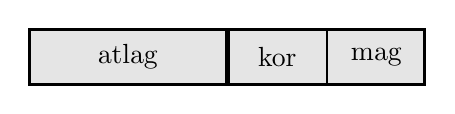
\begin{tikzpicture}
		\tikzstyle{Node} = [rectangle, minimum width=2.5cm, minimum height=7mm, text centered, draw=black, fill= gray!20, line width = 1.2pt]
		\tikzstyle{Border} = [rectangle, minimum width=2.5cm, minimum height=7mm, text centered, draw=black, line width = 1.2pt]
		\tikzstyle{HalfNode} = [rectangle, minimum width=1.25cm, minimum height=7mm, text centered, draw=black, fill= gray!20, line width = 0.2pt]
		\tikzstyle{arrow} = [thick,->,>=stealth]
		
		\node (1) [Node] {atlag};
		\node (2) [HalfNode, right = 0mm of 1] {kor};
		\node (3) [HalfNode, right = 0mm of 2] {mag};
		\node (border) [Border, right = -0.2mm of 1] {};
		
		\end{tikzpicture}
	\end{figure}
	Azaz, \texttt{atlag}, illetve \texttt{kor} és \texttt{magassag} pont efértek 1-1 gép szóban. Viszont, ha megcseréljük a sorrendet, ez már nem lesz igaz:
	\begin{figure}[H]
		\centering
		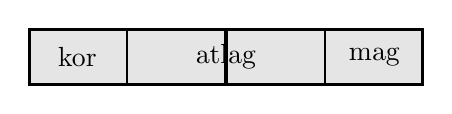
\begin{tikzpicture}
		\tikzstyle{Node} = [rectangle, minimum width=2.5cm, minimum height=7mm, text centered, draw=black, fill= gray!20]
		\tikzstyle{Border} = [rectangle, minimum width=2.5cm, minimum height=7mm, text centered, draw=black, line width = 1.2pt]
		\tikzstyle{HalfNode} = [rectangle, minimum width=1.25cm, minimum height=7mm, text centered, draw=black, fill= gray!20, line width = 0.2pt]
		\tikzstyle{arrow} = [thick,->,>=stealth]
		
		\node (1) [HalfNode] {kor};
		\node (2) [Node, right = 0mm of 1] {atlag};
		\node (3) [HalfNode, right = 0mm of 2] {mag};
		\node (border) [Border, right = -1.26cm of 1] {};
		\node (border) [Border, left = -1.26cm of 3] {};
		\end{tikzpicture}
	\end{figure}
	Sajnos itt már szétvágná \texttt{atlag}-ot. Ez nagyon nem hatékony, mert állandóan gondolnia kéne a fordítónak arra, hogy épp hogyan kaparja össze \texttt{atlag}-ot.
	\begin{figure}[H]
		\centering
		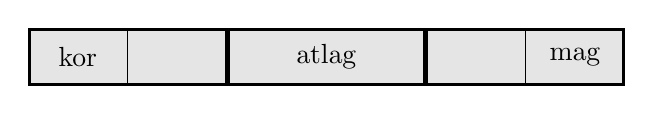
\begin{tikzpicture}
		\tikzstyle{Node} = [rectangle, minimum width=2.5cm, minimum height=7mm, text centered, draw=black, fill= gray!20, line width = 1.2pt]
		\tikzstyle{HalfNode} = [rectangle, minimum width=1.25cm, minimum height=7mm, text centered, draw=black, fill= gray!20, line width = 0.2pt]
		\tikzstyle{Border} = [rectangle, minimum width=2.5cm, minimum height=7mm, text centered, draw=black, line width = 1.2pt]
		\tikzstyle{arrow} = [thick,->,>=stealth]
		
		\node (1) [Node] {atlag};
		\node (2) [HalfNode, left = 0mm of 1] {};
		\node (3) [HalfNode, left = 0mm of 2] {kor};
		\node (4) [HalfNode, right = 0mm of 1] {};
		\node (5) [HalfNode, right = 0mm of 4] {mag};
		\node (border) [Border, right = -0.2mm of 1] {};
		\node (border) [Border, left = -0.2mm of 1] {};
		\end{tikzpicture}
	\end{figure}
	Ez így sokkal hatékonyabb, bár 3 gép szót használ. Ebben az esetben a kód eltárolja, hogy legyen egy kis \textit{padding } a változó után. Tehát semmi extráért nem kell fizetnünk, de attól még picit több memóriát foglalunk le.
	\smallskip
	
	A szabvány kimondja, hogy egy \texttt{struct} mérete az adottagok méreteinek összegénél nagyobbegyenlő.
	\smallskip
	
	Az, hogy egy gépi szó mekkora, implementációfüggő.
	\bigskip
	
	Egy \texttt{struct} egyes adattagjaira így hivatkozhatunk:
	\begin{lstlisting}
int main()
{
	//...
	Hallgato a;
	std::cout << a.kor << std::endl;
	Hallgato b = a;
	b.magassag = 3;
}
	\end{lstlisting}      
	
\end{document}
